\begin{anexosenv}

% Imprime uma página indicando o início dos anexos
\partanexos

% ---
\chapter{Pseudocódigo: algoritmo de avaliação de soluções}

novo Mapa Soluções;

adicionar árvore a Soluções;

nova Fila Soluções a avaliar;

enfilar árvore em Soluções a avaliar;

enquanto Soluções a avaliar não é vazia {

	nova Solução S1;
	tirar a primeira Solução da fila e atribuir à S1;
	transformar arvore utilizando as transformações de S1;
	nova Lista Nós a avaliar;
	criar Lista de nós para a raíz de S1 e atribuir à Nós a avaliar;
	novo Mapa Soluções por nó;
	para cada Nó N em Nós a avaliar {
		Soluções por nó recebe uma nova Lista em N;
		nova Lista Pré-soluções;
		combinar soluções dos filhos direito e esquerdo de N
			e atribuir a Pré-soluções;
		para cada Solução P em Pré-soluções {
			nova Solução S2 recebe a combinação de S1 e P;
			adicionar S2 à Lista no Soluções por nó em N;
			se N é raiz e a chave de S2 não está em Soluções {
				adicionar S2 a Soluções e Soluções a avaliar;
			}
			novo Nó H recebe N;
			nova Solução SH recebe S2;
			enaquanto H pode ser rotacionado no sentido horário {
				rotacionar H no sentido horário;
				adicionar transformação feita às transformações de SH;
				adicionar SH à Lista no Soluções por nó em N;
				se o pai de H é raiz e a chave de SH não está em Soluções {
					adicionar SH a Soluções e Soluções a avaliar;
				}
				atribuir o pai de H a H;
			}
			desfazer todas as rotações feitas no sentido horário;
			novo Nó AH recebe N;
			nova Solução SAH recebe S2;
			enaquanto AH pode ser rotacionado no sentido anti-horário {
				rotacionar AH no sentido anti-horário;
				adicionar transformação feita às transformações de SAH;
				adicionar SAH à Lista no Soluções por nó em N;
				se o pai de AH é raiz e a chave de SAH não está em Soluções {
					adicionar SAH a Soluções e Soluções a avaliar;
				}
				atribuir o pai de AH a AH;
			}
			desfazer todas as rotações feitas no sentido anti-horário;
			desfazer as transformações de P;
		}
	}
	desfazer as trasnformações de S1;
}

\chapter{Exemplo: mapa de execução do algoritmo de avaliação de soluções}

\begin{figure}[H]
% 	\caption{\label{gram_cls}Classes da Classificação de Chomsky e sua hierarquia}
	\begin{center}
	    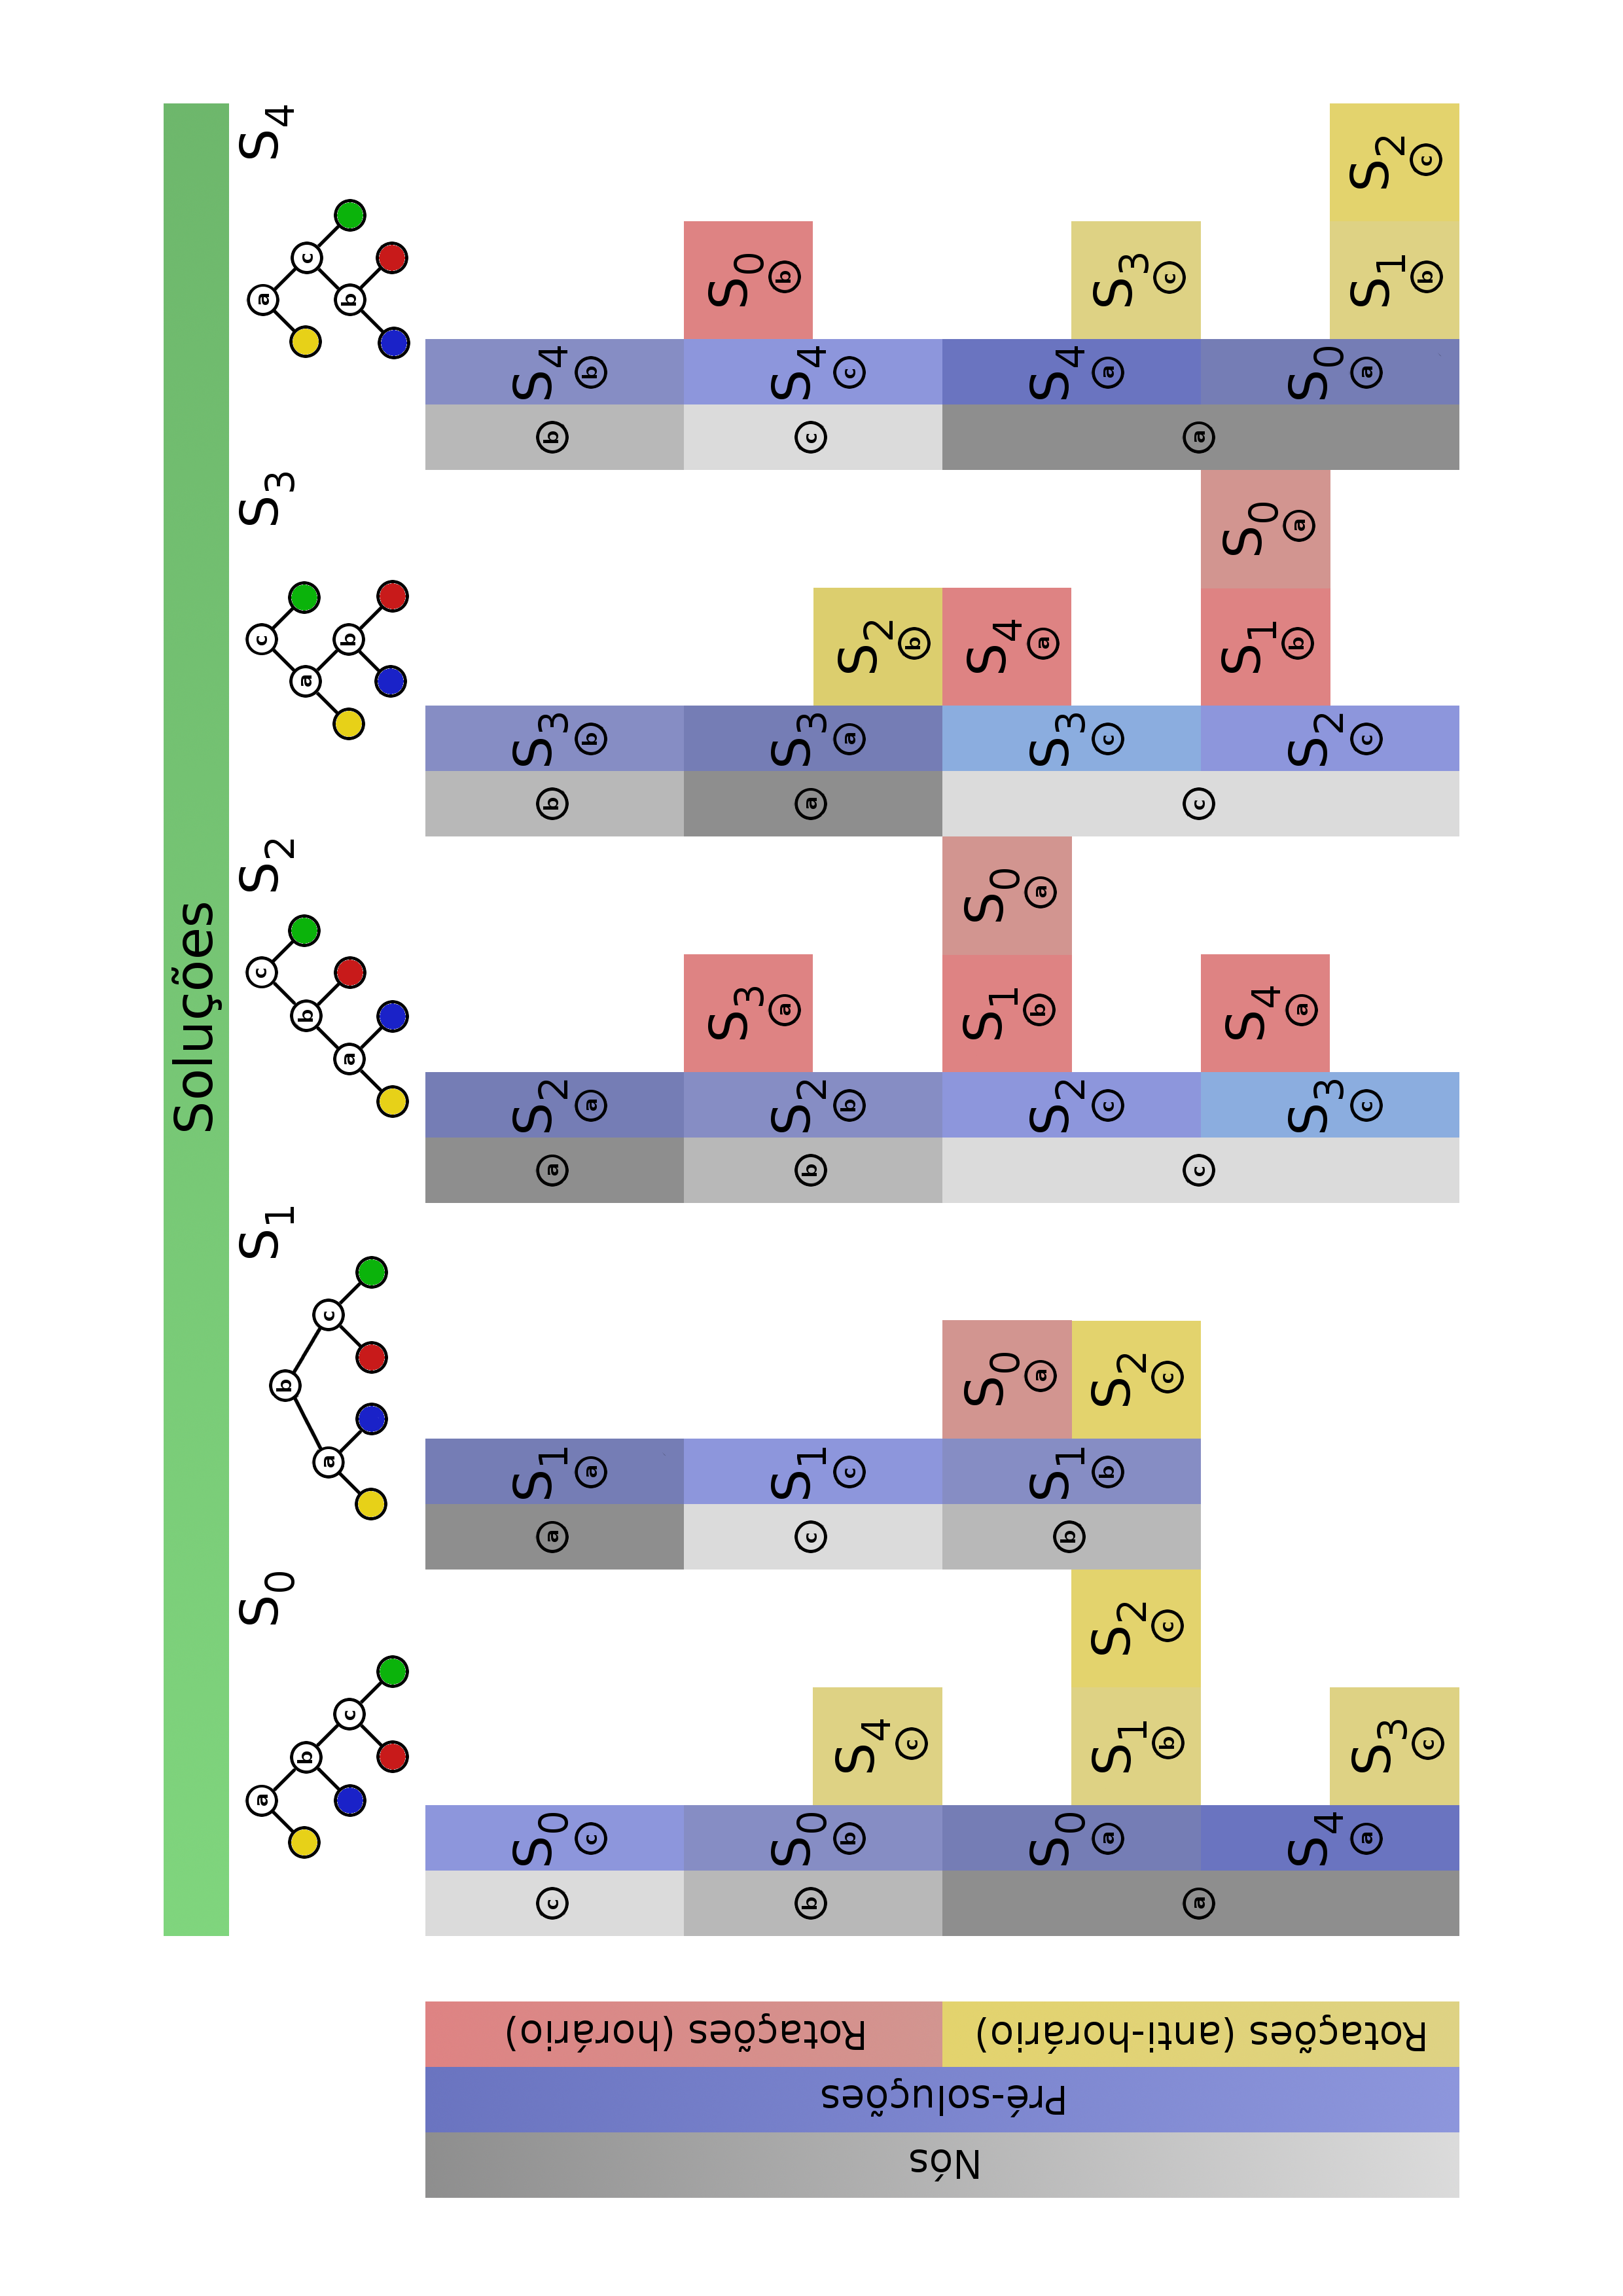
\includegraphics[scale=0.75]{alg_exp.png}
	\end{center}
% 	\legend{Fonte: Produzido pelo autor}
\end{figure}

\chapter{Gráfico: Tempos de execução do algoritmo de avaliação de soluções (escala linear)}

\begin{figure}[H]
	\begin{center}
	    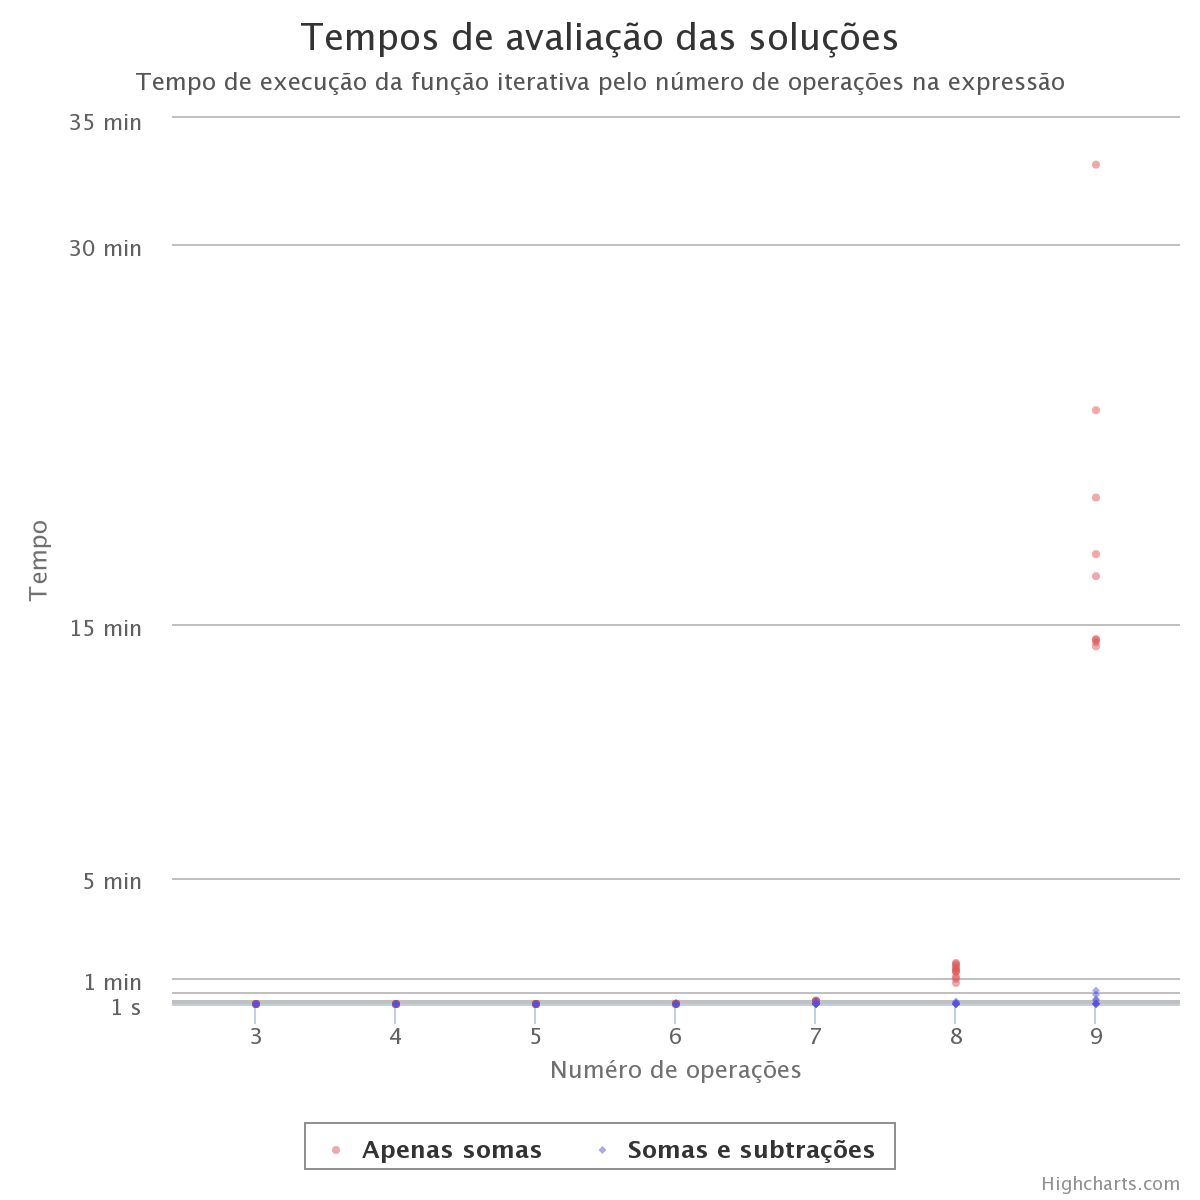
\includegraphics[scale=0.75]{timming_test_lin.png}
	\end{center}
\end{figure}

\chapter{Gráfico: Tempos de execução do algoritmo de avaliação de soluções (escala logarítmica)}

\begin{figure}[H]
	\begin{center}
	    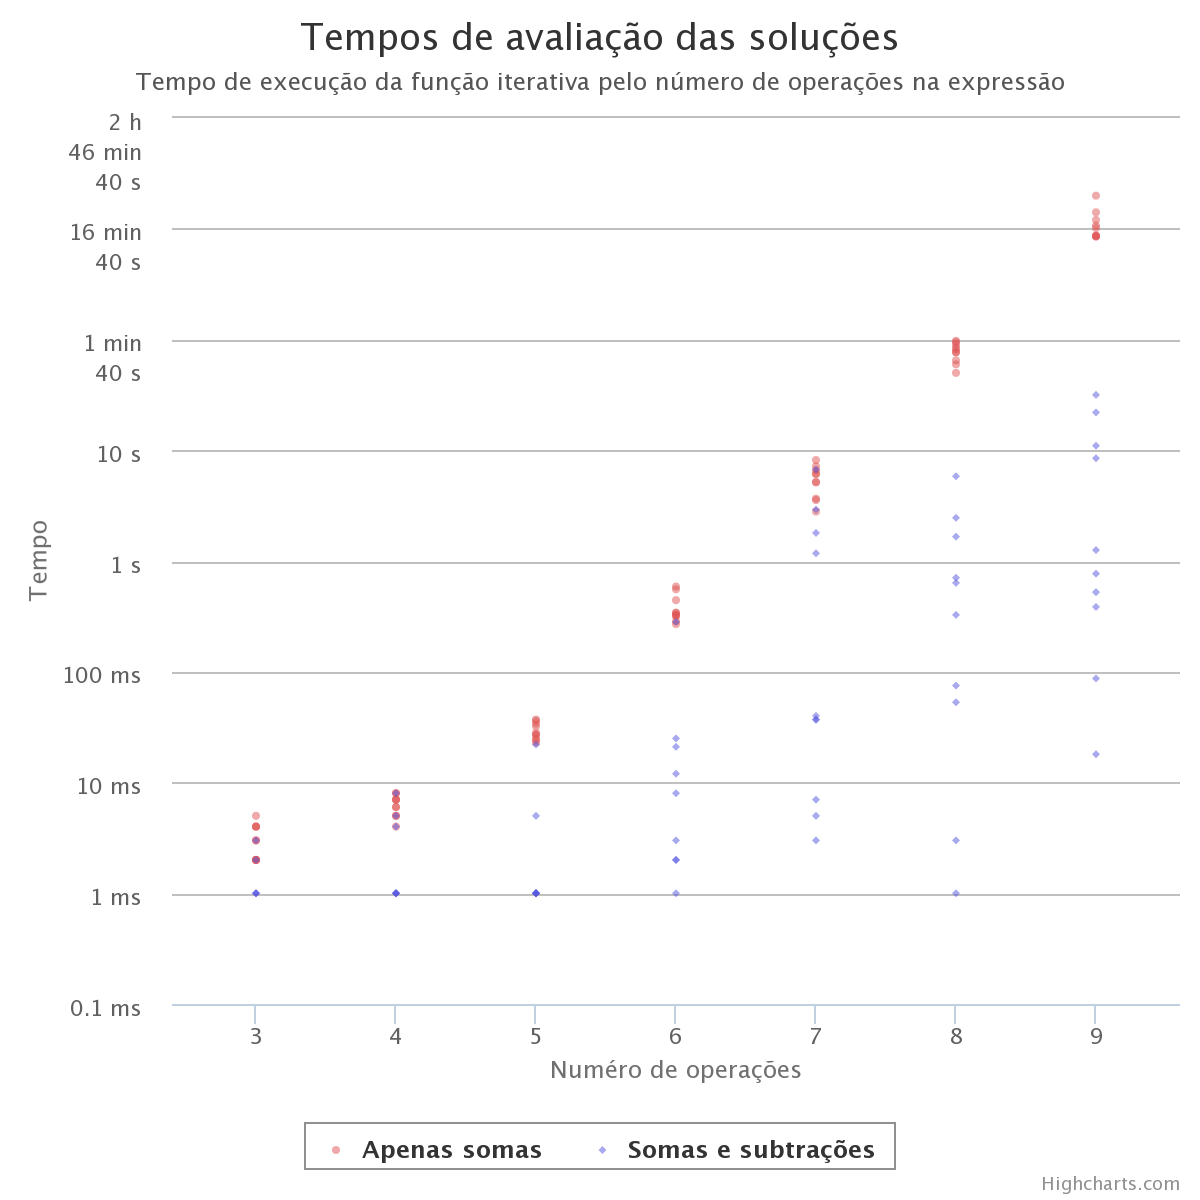
\includegraphics[scale=0.75]{timming_test_log.png}
	\end{center}
\end{figure}

\end{anexosenv}
